\documentclass{article}

% if you need to pass options to natbib, use, e.g.:
%     \PassOptionsToPackage{numbers, compress}{natbib}
% before loading neurips_2018

% ready for submission
% \usepackage{neurips_2018}

% to compile a preprint version, e.g., for submission to arXiv, add add the
% [preprint] option:
 % \usepackage[preprint]{neurips_2018}

% to compile a camera-ready version, add the [final] option, e.g.:
 \usepackage[final]{neurips_2019}
% to avoid loading the natbib package, add option nonatbib:
%     \usepackage[nonatbib]{neurips_2018}
\usepackage{graphicx}
\usepackage[utf8]{inputenc} % allow utf-8 input
\usepackage[T1]{fontenc}    % use 8-bit T1 fonts
\usepackage{hyperref}       % hyperlinks
\usepackage{url}            % simple URL typesetting
\usepackage{booktabs}       % professional-quality tables
\usepackage{amsfonts}       % blackboard math symbols
\usepackage{nicefrac}       % compact symbols for 1/2, etc.
\usepackage{microtype}      % microtypography
\usepackage{amsmath}
\usepackage{bm}
\usepackage{subfig}
\usepackage[english]{babel}
\usepackage{algorithm}
\usepackage{algorithmic}
\usepackage{appendix}
\newtheorem{theorem}{Theorem}
\newtheorem{lemma}{Lemma}
\newtheorem{proof}{Proof}
\input macros.tex
\title{Multi-way block localization vis sparse tensor clustering}

% The \author macro works with any number of authors. There are two commands
% used to separate the names and addresses of multiple authors: \And and \AND.
%
% Using \And between authors leaves it to LaTeX to determine where to break the
% lines. Using \AND forces a line break at that point. So, if LaTeX puts 3 of 4
% authors names on the first line, and the last on the second line, try using
% \AND instead of \And before the third author name.

\author{%
Yuchen Zeng \\
 University of Wisconsin -- Madison\\
 \texttt{yzeng58@wisc.edu} \\
\And
Miaoyan Wang \\
 University of Wisconsin -- Madison\\
\texttt{miaoyan.wang@wisc.edu} \\
%Madison, WI 53703 \\
% Affiliation \\
  % Address \\
  % \texttt{email} \\
  % \AND
  % Coauthor \\
  % Affiliation \\
  % Address \\
  % \texttt{email} \\
  % \And
  % Coauthor \\
  % Affiliation \\
  % Address \\
  % \texttt{email} \\
  % \And
  % Coauthor \\
  % Affiliation \\
  % Address \\
  % \texttt{email} \\
}

\begin{document}
% \nipsfinalcopy is no longer used

\maketitle

\begin{abstract}
 We consider the task of simultaneously clustering each mode of a large noisy tensor. We assume that the tensor elements are distributed with a block-specific mean and propose a least-square estimation for multi-way clustering. An $\ell_1$ penalty is applied to the block-means in order to select and identify important blocks. We show that our method is applicable to large tensors with a wide range of multi-way cluster structure, including a single block, multiple blocks, checkerboard clusters, 1-way or lower-way blocks. Our proposal amounts to a sparse, multi-way version of $k$-mean clustering, and a relaxation of our proposal yields the tensor Tucker decomposition. The performance of our proposals are demonstrated in simulations and on... 
\end{abstract}

\section{Introduction}
In recent years, much interest has centered around the unsupervised analysis of high-dimensional high-order tensor data. ....


Here is an example of tensor clustering by using our proposed method.
\begin{figure}[!h]
	\centering
	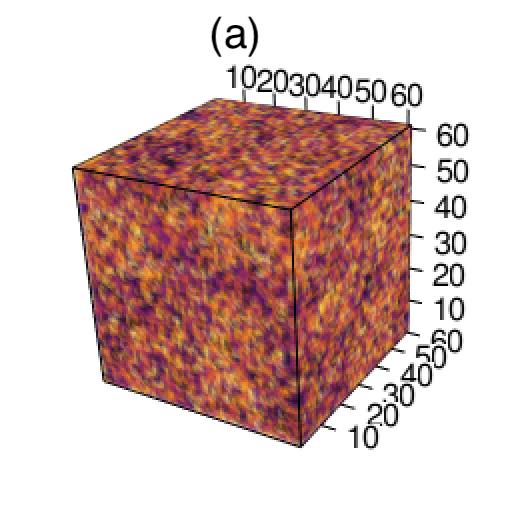
\includegraphics[scale=0.35]{figures/figure1/input.png}
	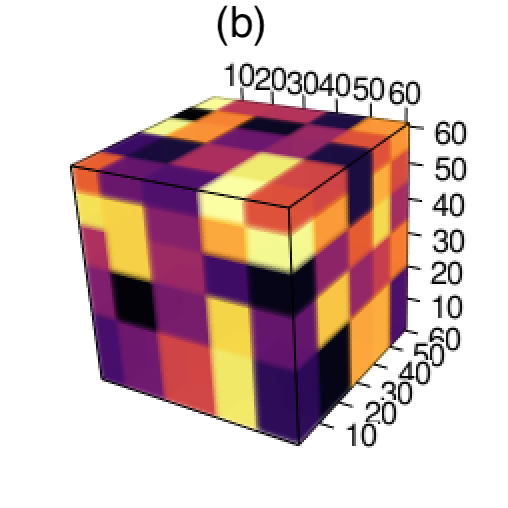
\includegraphics[scale=0.35]{figures/figure1/truth.png}
	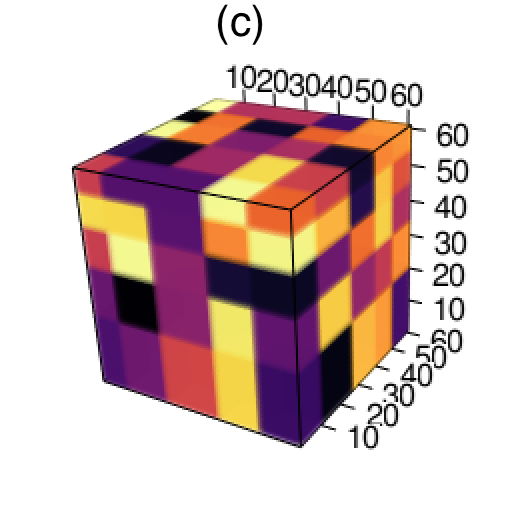
\includegraphics[scale=0.35]{figures/figure1/output.png}
	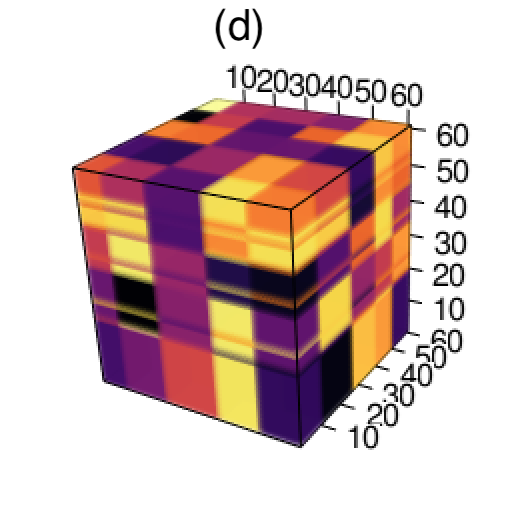
\includegraphics[scale=0.35]{figures/figure1/k_means.png}
	\caption{(a): a 60*60*60 tensor with 5 clusters in each mode; (b): true underlying mean signal within each cluster; (c): mean signal estimated by our proposed approach with true number of clusters: 5, 5, 5; (d): mean signal estimated by k-means clustering on each mode with true number of clusters:5 , 5, 5.}
	\label{fig1}
\end{figure}

\begin{figure}
	\centering
	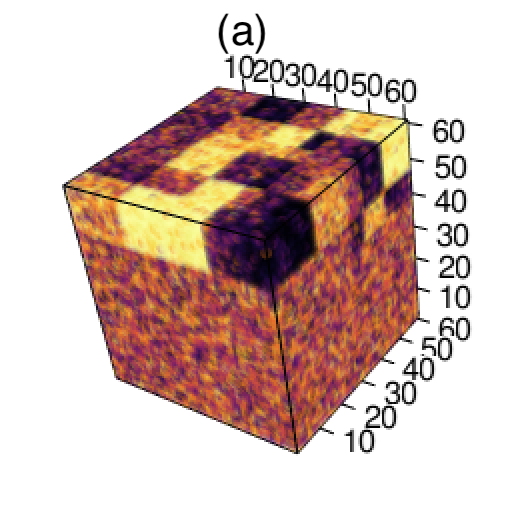
\includegraphics[scale=0.5]{figures/figure2/input.png}
	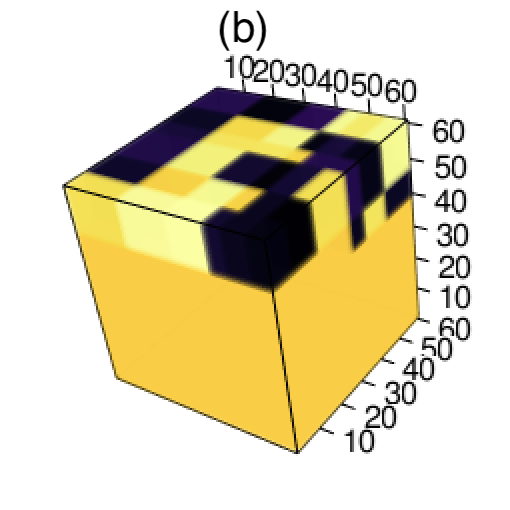
\includegraphics[scale=0.5]{figures/figure2/truth.png}
	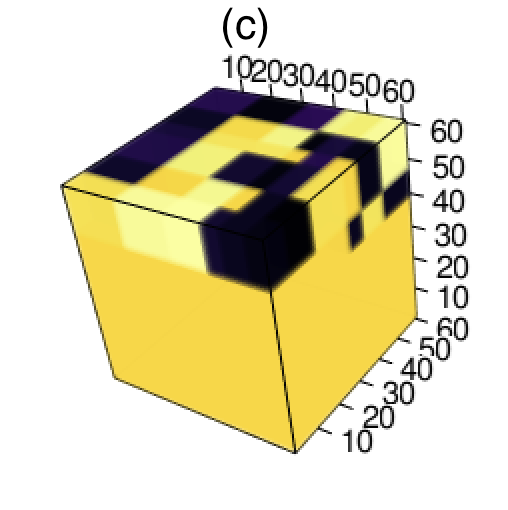
\includegraphics[scale=0.5]{figures/figure2/output.png}
	\caption{(a): 60*60*60 sparse tensor; (b) true underlying means; (c) mean signal estimated by our approach with estimated number of clusters and estimated $\lambda$.}
	\label{fig2}
\end{figure}
\subsection{Notation}
We use $\tT$, $\tX$, and $\tE$ to represent input, signal, and noise tensors, respectively. For any set $J$, $|J|$ denotes its cardinality. $[n]$ represents the set $\{1,2,\ldots,n\}$. $\mx\otimes \my$ is the Kronecker product of two vectors. 


\subsection{Problem formulation}
\textbf{Notations:}\\
1. $K$: the number of dimensions of the data;\\
2. $n_i$: the number of observations in the $i$th mode, $i=1,2,...,K$;\\
3. $d_i$: the number of clusters in the $i$th mode, $i=1,2,...,K$;\\
4. $c_{ij}$: the $j$th cluster of the $i$th mode, $i=1,2,...,K$, $j=1,...,d_i$;\\
5. $q$: the number of non-zero clusters;\\
%======================Wait for verify===================================
6. $c$: the degree of freedom while doing tensor clustering: $\sum_{i=1}^Kd_ilog(n_i)$;\\
%======================Wait for verify===================================
7. $S$: the rank while producing multiplicative data.
\section{Tuning Parameter Selection}
Before doing tensor clustering, we need to select appropriate tuning parameters. 
There are $K+1$ tuning parameters in our tensor clustering proposal: the number of clusters in each modes: $d_1$, $d_2$, ..., $d_K$ and the penalty coefficient $\lambda$. For both the number of clusters and the penalty coefficient, we try to use BIC and cross validation to find the best choice. It turns out the BIC is faster when the accuracy is almost the same, so we use BIC to select the tuning parameters. \par
\begin{equation*}
BIC = \prod_{i=1}^K n_i\times log(RSS)+(q+c)log(\prod_{i=1}^K n_i)
\end{equation*}

As for the number of clusters, given a range of $d_1$, $d_2$, ..., $d_K$, we do the tensor clustering for all combinations of $d_1$, $d_2$, ..., $d_K$ with $\lambda=0$ and calculate the BIC for each of them separately using the formula above. We choose the $d_1$, $d_2$, ..., $d_K$ which is the smallest among all combinations of $d_1$, $d_2$, ..., $d_K$ whose BIC is the smallest. \par

 After estimating the $d_1$, $d_2$, ..., $d_K$, we use the estimated number of clusters to do tensor clustering when given a reasonable range of $\lambda$. We perform the tensor clustering and calculate the BIC on all $\lambda$ in the given range. Then we select the smallest $\lambda$ with smallest BIC.

\section{Simulation and Evaluation}
For simplicity, we only consider the situation $K=3$ here. 
Given the approach of clustering in the former section, we will evaluate the performance of it in different aspects on non-sparse and sparse tensor. When the tensor is non-sparse, first, we would assess the relationship between MSE and the data size; second, we would verify the clustering approach when true $d_1$, ..., $d_K$ is given; third, we would evaluate the approach of estimating the number of clusters; fourth, we would evaluate the synergistic performance of selecting $d_1$, ..., $d_K$ and clustering; fifth, we would check the performance of our approach in a different kind of tensor and compare it with other clustering approach. As for sparse tensor, we would evaluate the whole process: selecting $d_1$, ..., $d_K$, choosing $\lambda$, doing tensor clustering.\par 

There are the statistics we would use to evaluate the performance in different cases:\\
(1) CER(clustering error rate): the adjusted rand index between two paritions. This statistic measure the agreement between the true partition and estimated partition of the data tensor. In this case, we have three kinds of CER in total: CER of mode 1, CER of mode 2 and CER of mode 3;\\
(2) Total Correct Rate: 1 - the proportion of misjudgement while determining whether the mean signal is zero.;\\
(3) Correct Zero Rate: the proportion of zero elements are correctly identified in the underlying mean tensor;\\
(4) Correct One Rate: the proportion of non-zero elements are correctly identified in the underlying mean tensor.\\
(5) Error: measuring the difference between the underlying means and the estimated means.\par  

In non-sparse cases, we mainly use CER as an indicator to judge whether our proposal methods are good or bad because it is more intuitive for us to evaluate the performance of our approach comparing with MSE. However, it has some constraints. In sparse cases, different clusters can have the same mean: 0. In this case, we can have multiple reasonable partitions of the modes. Thus, CER is inapplicable at this time and we use  total correct rate, correct zero rate and correct one rate to be the indicator when the tensor is sparse.
\par


Here we give a brief elaboration on the main way we use to generate the data. As for non-sparse tensor, given the cluster numbers $d_1$, ..., $d_K$ and the size of the tensor $n_1n_2n_3$, we assign the labels to each modes randomly. Next we randomly select the mean signal of clusters from Unif(-3,3) and add noise which comes from normal distribution with given standard deviation. Then we get the non-sparse tensor. As for sparse tensor, we randomly assign 0 to the mean of some  clusters with given sparsity rate (the proportion of 0 elements) and then follow the same steps. We name this kind of tensor as tensor with constant clusters.\par 

\textbf{Non-sparse case.} We begin with verifying the relationship between MSE and the sample size. The theoretical result indicates that the boundary of $RMSE=\sqrt{MSE}= \sqrt{\frac{error}{n_1n_2n_3}}$ decreases with respect to sample size. Here we let $n_1$ to take values from 20 to 70, and $n_2=\frac{n_1logd_1}{logd_2}$,, $n_3 = \frac{n_1logd_1}{logd_3}$. As for $d_1, d_2, d_3$, we take them from $\{(4,4,4),(4,8,8),(8,8,8),(8,8,12)\}$. We simulated each situation 50 times and get the average RMSE among those cases. According to the panel (a) of Figure \ref{fig3}, obviously, with sample size going up, the RMSE goes down. Additionally, the panel (b) of Figure \ref{fig3} indicates the RMSE decreases roughly at the rate of $1/N$ where $N=\sqrt{n_2n_3/logd_1}$ is the rescaled sample size.\par 

\begin{figure}
	\centering
	\subfloat[]{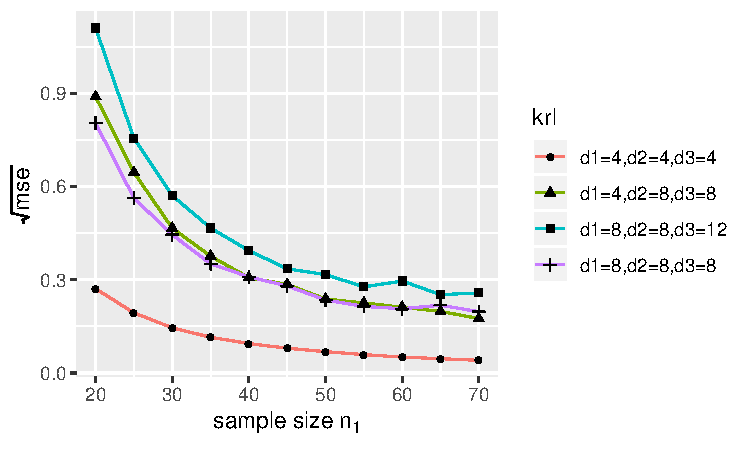
\includegraphics[scale=0.5]{figures/figure3/non-scale.pdf}}
	\subfloat[]{
\includegraphics[scale=0.5]{figures/figure3/rescale.pdf}}
	\caption{Plots of the root mean squared error (RMSE) verus sample size when using our tensor clustering algorithm. Each curve corresponds to a fixed $(d_1,d_2,d_3)$. (a): Plots of average RMSE over 50 simulations against $n_1$; (b): Plots of averge RMSE over 50 simulations against $\sqrt{n_2n_3/logd_1}$. }
	
	\label{fig3}
\end{figure}

In the second simulation, we generate 50 non-sparse tensors with the same noise, size and cluster numbers each time. We use our approach (Algorithm \ref{alg:B}) to do the clustering and the result is shown as Table \ref{t1}. In both data size: 40*40*40 and 40*40*80, the CER on all modes are 0 when the noise is 4. As the noise goes up, the CER is increased gradually. Furthemore, from the $d_1=3, d_2=5, d_3=4$ cases, we notice that the CER of mode $i$ seems to be smaller when the number of clusters in the $i$th mode is less. \par 

\begin{table}
	\centering
	\begin{tabular}{|c|c|c|c|c|c|c|c|c|c|}
		\hline
		$n_1$&$n_2$&$n_3$&$d_1$&$d_2$&$d_3$&noise&CER (mode 1)&CER (mode 2)&CER (mode 3)\\ \hline
		40&40&40&3&5&4&4&
		$\mathbf{0(0)}$&$\mathbf{0(0)}$&$\mathbf{0(0)}$\\
		40&40&40&3&5&4&8&$\mathbf{0(0)}$&0.0095(0.0247)&0.0021(0.0145) \\
		40&40&40&3&5&4&12&0.0038(0.0138)&0.0331(0.0453)&0.0222(0.0520)\\

		40&40&80&3&5&4&4&$\mathbf{0(0)}$&0.0017(0.0121)&$\mathbf{0(0)}$\\
		40&40&80&3&5&4&8&$\mathbf{0(0)}$&$\mathbf{0(0)}$&$\mathbf{0(0)}$\\
		40&40&80&3&5&4&12&$\mathbf{0(0)}$&$0.0257(0.0380)$&$0.0026(0.0064)$\\

		40&40&40&4&4&4&4&$\mathbf{0(0)}$&$\mathbf{0(0)}$&$\mathbf{0(0)}$\\
		40&40&40&4&4&4&8&0.0023(0.0165)&0.0034(0.0239)&$\mathbf{0(0)}$\\
		40&40&40&4&4&4&12&0.0519(0.0744)&0.0414(0.0697)&0.0297(0.0644)\\
		
		40&40&80&4&4&4&4&$\mathbf{0(0)}$&$\mathbf{0(0)}$&$\mathbf{0(0)}$\\
		40&40&80&4&4&4&8&$\mathbf{0(0)}$&$\mathbf{0(0)}$&$\mathbf{0(0)}$\\
		40&40&80&4&4&4&12&0.0132(0.0405)&0.0106(0.0366)&0.0043(0.0168) \\
		\hline
	\end{tabular}
	\caption{Given the true $d_1,d_2,d_3$, the simulation results is calculated across 50 tensors each time. }
	\label{t1}
\end{table}


To evaluate the performace of our approach on selecting the number of clusters, we generate 50 non-sparse tensors with the same noise, size and cluster numbers in each case in Table \ref{t2} as the third simulation.  The reason why we only evaluate the performance of estimation on cluster numbers on non-sparse tensor is in sparse case, the reasonable cluster numbers may not be unique. As expected, we achieve 100\% accuracy when the noise is 4, again. The overall accuracy goes down as the noise increased. Additionally, we notice that the smaller $d_i$ is, the more accurate the estimated value is. There are two extremely low overall accuracy which appears when noise is 12 and the tensoe size is 40*40*40. However, the accuracy is improved quickly as the tensor size is enlarged to 40*40*80. We found that not only the accuracy of mode 3 decreased after we add observations on mode 3, but also the accuracy of other two modes decreased a lot. The reason is the length of an observation in mode 1 and mode 2 is longer than before. Therefore, it is very important for us to get enough observations to guarantee the overall accuracy.\par

\begin{table}
	\centering
	\resizebox{\textwidth}{20mm}{
	\begin{tabular}{|c|c|c|c|c|c|c|c|c|c|c|}
		\hline
		$n_1$&$n_2$&$n_3$&$d_1$&$d_2$&$d_3$&noise&overall accuracy&estimated $d_1$&estimated $d_2$&estimated $d_3$\\ \hline
		40&40&40&3&5&4&4&$\mathbf{1}$&3(0)&5(0)&4(0)\\
		40&40&40&3&5&4&8&0.74&3(0)&4.76(0.0610)&3.98(0.02)\\
		40&40&40&3&5&4&12&0.02&2.8(0.0571)&3.58(0.1072)&3.3(0.0915)\\
		40&40&40&4&4&4&4&$\mathbf{1}$&4(0)&4(0)&4(0)\\
		40&40&40&4&4&4&8&0.88&3.94(0.0339)&3.96(0.0280)&3.96(0.0280)\\
		40&40&40&4&4&4&12&0.04&3.08(0.0983)&3.12(0.1016)&3.12(0.0975)\\
		40&40&80&4&4&4&4&$\mathbf{1}$&4(0)&4(0)&4(0)\\
		40&40&80&4&4&4&8&1&4(0)&4(0)&4(0)\\
		40&40&80&4&4&4&12&0.78&3.9(0.0429)&3.92(0.0388)&3.96(0.04)\\
		\hline
	\end{tabular}}
	\caption{The simulation results across 50 tensors each time from estimating the $d_1,d_2,d_3$.}
	\label{t2}
\end{table}

In the forth simulation, the true cluster numbers are not given, so we estimate them first and then use the estimated true cluster numbers to estimate the parition of clusters as well as underlying mean signals. We set the true cluster numbers to be $d_1=3, d_2=5, d_3=4$ specifically here, and the results are shown in Table \ref{t3}. By looking into each mode separately, as the sample size of that mode increased , the CER of that mode decreased without any exception.\par  
\begin{table}
	\centering
	\begin{tabular}{|c|c|c|c|c|c|c|}
		\hline
		$n_1$&$n_2$&$n_3$&noise&CER(mode 1)&CER(mode 2)&CER(mode3)\\ \hline
		40&40&40&4&$\mathbf{0(0)}$&$\mathbf{0(0)}$&$\mathbf{0(0)}$\\
		40&40&40&8&$\mathbf{0(0)}$&0.0136(0.0226)&0.0005(0.0036) \\
		40&40&40&12&0.0365(0.0789)&0.12(0.0878)&0.0802(0.1009)\\
		40&45&50&4&$\mathbf{0(0)}$&$\mathbf{0(0)}$&$\mathbf{0(0)}$\\
		40&45&50&8&$\mathbf{0(0)}$&0.0027(0.0121)&$\mathbf{0(0)}$\\
		40&45&50&12&0.0158(0.0489)&0.0641(0.0629)&0.0336(0.0647)\\
		\hline
	\end{tabular}
	\caption{The CERs over 50 simulated tensors ($d_1=3, d_2=5, d_3=4$) each time.}
	\label{t3}
\end{table}

In the fifth simulation, we generate the tensor in two different ways. The new way to generate data is using $\sum_{s=1}^{S}d_s\mathbf{u_s}\mathbf{v_s}^T$ after giving the $S$.  First we randomly choose $\mathbf{u_s}$ and $\mathbf{v_s}$ from normal distribution where $i=1,...,S$. Then we add noise which is also sampled from normal distribution with given standard deviation. We name the tensor generated in this way as tensor with multiplicative clusters. In this simulation, we would check whether our method is still robust on the tensors with multiplicative cluster. Meanwhile, we would compare the performance of our approach with CPD k-means (do k-means clustering after using CP decomposition on the data tensor) under different noise and different kinds of tensor. To be more specific, when the data a a tensor with  multiplicative clusters we just use the true rank that we use to generate the data tensor to do the CP k-means. As for the parameter $d_1, d_2, d_3$ in kmeans, we also use the true parameter. We apply the true $d_1, d_2, d_3$ in our method, too. When the data is a tensor with constant clusters, we still use true $d_1, d_2, d_3$ in both methods. But for CPD k-means, we use BIC to select the best $S$ according to the formula: $error+\frac{log(n_1n_2n_3)(n_1+n_2+n_3-2)S}{n_1n_2n_3}$.  Here we set  $n_1=50,n_2=50,n_3=50$ and $d_1=4,d_2=4,d_3=4$ in all the cases, and add noise 0,10,20 to generate the tensors. Additionally, as for tensor with constant clusters, I randomly select underlying signals between -3 and 3; as for tensors with multiplicative clusters, I randomly select the elements of $\mathbf{u_s}$ and $\mathbf{v_s}$ between -3 and 3. Thus the mean signal of tensor with multiplicative clusters would be bigger than that of tensors with constant clusters. Therefore, the same noise would have bigger effect on the tensor with constant clusters. Our result is shown in Figure \ref{fig4}. To our surprise, our approach is not only better at working on tensor with constant clusters, but also better at working on tensor with multiplicative clusters. Furthermore, our approach shows more robustness under different level of noise, too. \par 

\begin{figure}
	\centering
	\subfloat[]{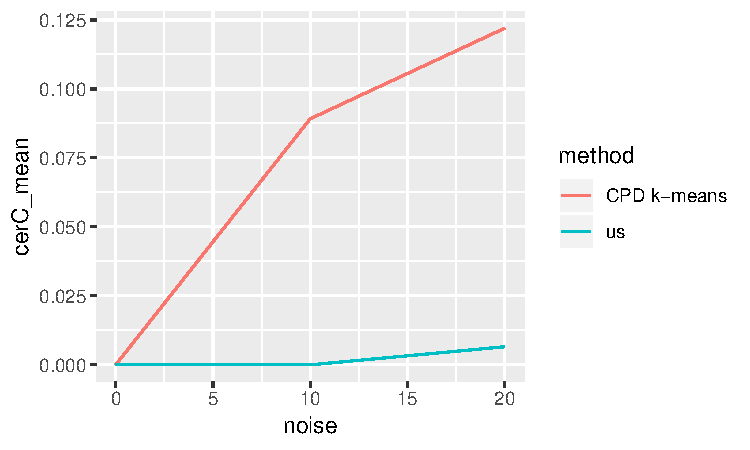
\includegraphics[scale=0.5]{figures/figure4/multidata.pdf}}
	\subfloat[]{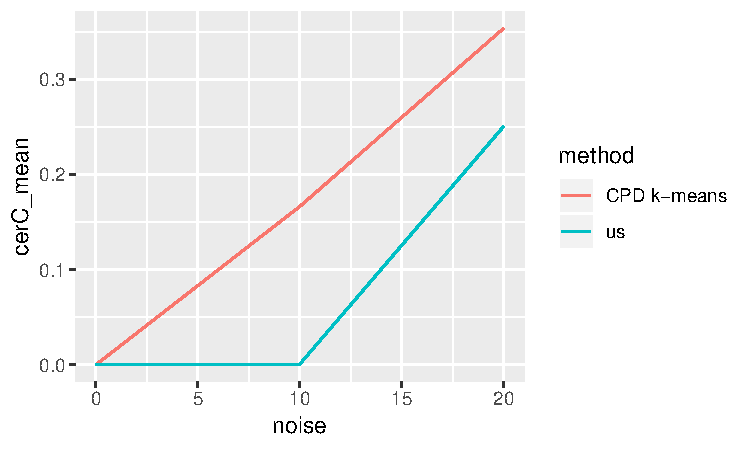
\includegraphics[scale=0.5]{figures/figure4/constantdata.pdf}}
	\caption{Plots of the mean CER C verus noise when using our tensor clustering algorithm and CPD k-means where $n_1=n_2=n_3=50, d_1=d_2=d_3=4$. Each curve corresponds to different method. (a): Plots of average CER in mode 1 over 50 simulations against noise while the  data is a tensor with multiplicative clusters where $S=3$; (b): Plots of averge CER in mode 1 over 50 simulations against noise while the data is a tensor with constant clusters.}
	\label{fig4}
\end{figure}



\textbf{Sparse case.} We also test the performace of our approach under different $\lambda$ when the data is sparse. The $\bar{\lambda}$ in Table \ref{t5} is the mean $\lambda$ we choose across 50 simulations on the same sparsity rate. According to Table \ref{t5}, the correct zero rate is increased with the increment on $\lambda$ while the correct one rate is exactly the opposite. As for the $\lambda$ we choose, it shows that the lowest total correct rate is 0.8586, which appears when noise is 8 and sparsity rate is 0.8. Overall, the $\lambda$ we select by BIC is fairly good, which does works better than other $\lambda$.

\begin{table}
	\centering
	\resizebox{\textwidth}{20mm}{
	\begin{tabular}{|c|c|c|c|c|c|c|}
		\hline
		sparsity rate&noise&method&estimated sparsity Rate&Correct Zero Rate&Correct One Rate&Total Correct Rate  \\ \hline
		0.5&4&$\lambda=0$&0(0)&0(0)&1(0)&0.5075(0.0676)\\
		0.5&4&$\lambda=100$&0.5677(0.0667)&1(0)&0.8519(0.0678)&0.9248(0.0377)\\
		0.5&4&$\lambda=200$&0.5952(0.0688)&1(0)&0.7975(0.0787)&0.8973(0.0433)\\
		0.5&4&$\bar{\lambda}=86.61396$&0.5606(0.0668)&$\mathbf{0.9993(0.0035)}$&$\mathbf{0.8655(0.0685)}$&$\mathbf{0.9312(0.0377)}$\\
		0.5&8&$\lambda=0$&0(0)&0(0)&1(0)&0.5075(0.0676)\\
		0.5&8&$\lambda=100$&0.5072(0.068)&0.879(0.0898)&0.8554(0.0634)&0.8665(0.0559)\\
		0.5&8&$\lambda=200$&0.5884(0.0618)&0.9753(0.034)&0.7877(0.0776)&0.8794(0.0492)\\
		0.5&8&$\bar{\lambda}=344.3656$&0.6298(0.0652)&0.9956(0.0128)&0.7259(0.0873)&0.8586(0.0518)\\
		0.8&8&$\lambda=0$&0(0)&0(0)&1(0)&0.2029(0.0541)\\
		0.8&8&$\lambda=100$&0.6458(0.0646)&0.7453(0.0616)&0.7136(0.2017)&0.7435(0.0668)\\
		0.8&8&$\lambda=200$&0.7947(0.0627)&0.9119(0.0601)&0.6259(0.2376)&0.8589(0.0698)\\
		0.8&8&$\bar{\lambda}=246.9212$&0.826(0.0622)&0.9462(0.0412)&0.6077(0.2495)&0.8841(0.0602)\\
		\hline
	\end{tabular}}
	\caption{Results for Simulation 6 over 50 simulated data sets ($n_1=40, n_2=40, n_3=40,  d_1=3, d_2=5, d_3=4$.}
	\label{t5}
\end{table}


\section*{References}

References follow the acknowledgments. Use unnumbered first-level heading for
the references. Any choice of citation style is acceptable as long as you are
consistent. It is permissible to reduce the font size to \verb+small+ (9 point)
when listing the references. {\bf Remember that you can use more than eight
  pages as long as the additional pages contain \emph{only} cited references.}
\medskip

\small

[1] Alexander, J.A.\ \& Mozer, M.C.\ (1995) Template-based algorithms for
connectionist rule extraction. In G.\ Tesauro, D.S.\ Touretzky and T.K.\ Leen
(eds.), {\it Advances in Neural Information Processing Systems 7},
pp.\ 609--616. Cambridge, MA: MIT Press.

[2] Bower, J.M.\ \& Beeman, D.\ (1995) {\it The Book of GENESIS: Exploring
  Realistic Neural Models with the GEneral NEural SImulation System.}  New York:
TELOS/Springer--Verlag.

[3] Hasselmo, M.E., Schnell, E.\ \& Barkai, E.\ (1995) Dynamics of learning and
recall at excitatory recurrent synapses and cholinergic modulation in rat
hippocampal region CA3. {\it Journal of Neuroscience} {\bf 15}(7):5249-5262.

\begin{appendices}
	\section{Lemma and Theorems}
	\begin{lemma}
		Let $\mathbf{Y} \in \mathbb{R}^n$ be a response vector and $\mathbf{X} \in \mathbb{R}^{n\times p}$ the design matrix. Assume the response vector $\mathbf{Y}$ is mean-centered, i.e., $\sum_iY_i=0$. Suppose that $\mathbf{X}$ is an orthogonal design matrix with $X^TX=diag(n_1,...,n_p)$. Define the ordinary least-square estimate $\hat{\bm{\beta}}_{ols} = (\hat{\beta}_{ols,1},...,\hat{\beta}^T_{ols,p})^T$. Consider the following constrained optimization: 
		\begin{equation*}
		\bm{
			\hat{\beta}} = argmin\{\frac{1}{2}||\mathbf{Y}-\mathbf{X}\bm{\beta}||^2_2+\lambda pen(\bm{\beta})\}
		\end{equation*}
		1. Case 1: L-0 penalization. $pen(\bm{\beta}) = ||\bm{\beta}||_0$:\\
		Under the change of tuning parameter $\lambda' := f(\lambda)=\sqrt{2\lambda}$  such that $\bm{\hat{\beta}} = (\hat{\beta}_1,..., \hat{\beta}_p)^T$ has a closed-form solution:
		\begin{equation*}
		\hat{\beta}_i = \hat{\beta}_{ols,i}\mathbb{I}_{|\hat{\beta}_{ols,i}|>\frac{\lambda'}{\sqrt{n_i}}}\ for\ all\ i=1,...,p
		\end{equation*}
		2. Case 2: L-1 penalization. $pen(\bm{\beta})= ||\bm{\beta}||_1$:\\
		$\bm{\hat{\beta}} = (\hat{\beta}_1,..., \hat{\beta}_p)^T$ has a closed-form solution:
		\begin{equation*}
		\hat{\beta}_i = sign(\hat{\beta_{ols,i}})(|\hat{\beta_{ols,i}}|-\frac{\lambda}{n_i})_+\ for\ all\ i=1,2,...,p
		\end{equation*}
		
	\end{lemma}
	\begin{proof}
		The thing we want to minimize is
		\begin{equation*}
		L=\frac{1}{2}||\mathbf{Y-X}\bm{\beta}||^2_2+\lambda||\bm{\beta}_0||=\frac{1}{2}(\mathbf{Y-X}\bm{\beta})^T(\mathbf{Y-X}\bm{\beta})+\lambda ||\bm{\beta}||_0=L_1+L_2
		\end{equation*} 
		where $L_1=\frac{1}{2}(\mathbf{Y-X}\bm{\beta})^T(\mathbf{Y-X}\bm{\beta})$, $L_2=\lambda ||\bm{\beta}||_0$. 
	
	\textbf{Case 1:}\par 
	 Here we view the optimization problem as a case in linear regression. 
	The $L_1$ is exactly the $RSS/2$ in this case. So we compare the increment of $L_1$  when $L_2$ takes different values. We denote $z$ as the number of  non-zero elements in $\bm{\beta}$.\\
	(1) Consider the case we have no constraint on $z$. Thus we only have to minimize $L_1$. By the knowledge of linear regression, we know the unique minimizer is $\bm{\hat{\beta}_{ols}}=\mathbf{(X^TX)^{-1}XY}$. Assume there are $m$ zero elements in $\bm{\hat{\beta}_{ols}}$ where $0\leq m \leq p$ \\
	(2) Consider the case we have constraint on $z$: $z = i$, where $i=0,1,2,...,m$. Obviously, among these cases the $L$ can be minimized if and only if $i=m$. So, $z=m$ and $\bm{\hat{\beta}}=\bm{\hat{\beta}_{ols}}$ is the minimizer of $L$ when $0\leq z\leq m$.
	(3) Consider the case that we have constraint on $x$: $z=m+1$. Then we have to take one more non-zero element in $\bm{\beta}$ to be zero. Suppose we take $\hat{\beta}_l \neq 0$ to be 0. Then we obtain 
	\begin{equation*}
		2L_1 -SSE(\beta_1,...,\beta_{l-1},\beta_{l+1},...,\beta_p)=SSR(\beta_l)
	\end{equation*}
	by the columns in $\mathbf{X}$ are orthogonal to each other. Additionally,
	\begin{equation*}
		SSR(\beta_l) = \mathbf{Y}^T(\mathbf{H-H_l})\mathbf{Y} 
	\end{equation*}
	where $\mathbf{H=X(X^TX)^{-1}X}=\sum_{i=1}^p\frac{1}{n_i}\mathbf{x_{(i)}x_{(i)}^T}$, $\mathbf{H_l} = \sum_{i\neq j}\mathbf{x_{(i)}x_{(i)}^T}$, $\hat{\beta}_l = \frac{1}{n_l}\mathbf{x_{l}Y}$. Thus, we can simplify the second equation as:
	\begin{equation*}
		SSR(\beta_l) = n_l\hat{\beta}_l^2
	\end{equation*}
	Thus, by taking $\hat{\beta}_l$ as 0, there is $\frac{n_l\hat{\beta}_l^2}{2}$ increment on $L_1$, $\lambda$ decrement on $L_2$. Obviously, if the increment of $L_1$ is larger than the decrement $L_2$, we should not take $\hat{\beta_l}$ as 0; conversely, if the increment of $L_1$ is less than the decrement of $L_2$, taking $\hat{\beta_l}$ as 0 can lessen the L.\\
	(4) As we discussed, if there is still at least one element in $\bm{\beta_k}$ that satisfies that $\frac{n_k\hat{\beta}_k^2}{2}\leq\lambda$, we can keep reducing $L$ by taking $\bm{\beta_k}$ as 0 until all remain non-zero elements in $\hat{\beta}$ do not satisfy $\frac{n_k\hat{\beta}_k^2}{2}\leq\lambda$. Then we can minimize $L$.\par 
	Over all, the $\bm{\beta}$ that minimized $L$ is:
	\begin{equation*}
			\hat{\beta}_i = \hat{\beta}_{ols,i}\mathbb{I}_{|\hat{\beta}_{ols,i}|>\frac{\lambda'}{\sqrt{n_i}}}\ for\ all\ i=1,...,p
	\end{equation*}
	
\textbf{Case 2:}\par
Here we use the properties of subderivative. Taking subderivative of $L$, we obtain
	
\begin{equation*}
\frac{\partial L}{\partial \beta_j} = 
\begin{cases}
\{n_j\beta_j-\mathbf{x_{(j)}^TY}+\lambda\} &\mbox{if $\beta_j>0$}\\
 [n_j\beta_j-\mathbf{x_{(j)}^TY}-\lambda, n_j\beta_j-\mathbf{x_{(j)}^TY}+\lambda]&\mbox{if $\beta_j=0$}\\
\{n_j\beta_j-\mathbf{x_{(j)}^TY}-\lambda\} &\mbox{if $\beta_j<0$}\\
\end{cases}
\end{equation*}
Because $\beta_j$ minimize $L$ if and only if $0 \in \frac{\partial L}{\partial \beta_j}$ and  $\mathbf{X}$ is orthogonal, we get:
\begin{equation*}
\hat{\beta_j} = 
\begin{cases}
\frac{\mathbf{x_{(j)}^TY}+\lambda}{n_j}&\mbox{if $\hat{\beta_j}<0$}\\
0 &\mbox{if $\hat{\beta_j}=0$}\\
\frac{\mathbf{x_{(j)}^TY}-\lambda}{n_j}&\mbox{if $\hat{\beta_j}>0$}\\
\end{cases}
\end{equation*}
Here, $\bm{\hat{\beta}}_{ols} = \mathbf{(X^TX)^{-1}X^TY} = diag(1/n_1, ..., 1/n_p)X^TY$, so $\hat{\beta}_{ols,j}=\frac{\mathbf{x_{(j)}^TY}}{n_j}$. Then the solution of $\hat{\beta_j}$ can be simplified as:
\begin{equation*}
	\hat{\beta}_i = sign(\hat{\beta_{ols,i}})(|\hat{\beta_{ols,i}}|-\frac{\lambda}{n_i})_+\ for\ all\ i=1,2,...,p
\end{equation*}
\end{proof}
	\section{Algorithm}
	\begin{algorithm}
		\caption{Block Localization}
		\label{alg:B}
		\begin{algorithmic}
			\STATE {Initialize $c_{11}, c_{12},...,c_{1d_1}$, $c_{21}, c_{22},...,c_{2d_2}$ and $c_{K1}, c_{K2},...,c_{Kd_K}$ by performing one-way k-means clustering on the columns and on the rows of the data matrix $X$.}
			\REPEAT 
			\FOR{i in \{1,2,...,K\}}
			\STATE (a) holding the clusters of all modes fixed, solve $\bm{\mu}$ by minimizing the loss function with L-0 penalty on $\bm{\mu}$, that is,
			$\mu_{r_1,r_2,...,r_K} = S(\frac{\sum_{i=1}^K\sum_{l_i\in c_{r_i}}X_{l_1,l_2,...,l_K}}{\prod_{i=1}^{K}|c_{r_i}|},\frac{\sqrt{2\lambda}}{\sqrt{\prod_{i=1}^{K}|c_{r_i}|}})$
			\STATE (b) holding  $\bm{\mu}$ and the clusters of other $i-1$ modes fixed, minimizing the loss function with L-0 penalty with respect to $c_{i,1},...c_{i,d_i}$ by assigning each observation in mode $i$ to the cluster in mode $i$ whose mean signal is closet to it.
		\ENDFOR
			\UNTIL{Convergence} 
		\end{algorithmic}
	\end{algorithm}

\end{appendices}
\end{document}
